%&documentstructuur
\documentclass[presentatie.tex]{subfiles}

\begin{document}
    \section{Documentstructuur}
    \clearrecentlist

    \begin{saveblock}{baseDocumentPart1}
        \begin{highlightblock}[linewidth=0.5\textwidth,gobble=12,frame=t]
            \documentclass{article}
        \end{highlightblock}
    \end{saveblock}

    \begin{saveblock}{baseDocumentPart2}
        \begin{highlightblock}[linewidth=0.5\textwidth,gobble=12,frame=none]
            \usepackage[utf8]{inputenc}
    
        \end{highlightblock}
    \end{saveblock}

    \begin{saveblock}{baseDocumentPart3}
        \begin{highlightblock}[linewidth=0.5\textwidth,gobble=12,frame=none]
            \title{My document}
            \author{Vincent Kuhlmann}
            \date{1 May 2021}
        \end{highlightblock}
    \end{saveblock}

    \begin{saveblock}{baseDocumentPart4}
        \begin{highlightblock}[linewidth=0.5\textwidth,gobble=12,frame=b]
            \begin{document}
            \maketitle
            \section{Introduction}
    
            Hallo iedereen!
            \end{document}
        \end{highlightblock}
    \end{saveblock}
    
   	\addtorecentlist{preamble}
    \begin{frame}
        \frametitle{Simpel document}
    
        \begin{columns}
            \begin{column}{0.5\textwidth}
                % \adjustbox{valign=T,raise={-0.1cm}}{
                %     %\vspace{2.1cm+10pt}
                %     A\,\vrule width 1pt height 1em\relax
                % }
                %\rlap{\adjustbox{valign=T}{\useblock{baseDocument}}}
                \useblock{baseDocumentPart1}\vspace{-5px}
                \useblock{baseDocumentPart2}\vspace{-5px}
                \useblock{baseDocumentPart3}
                \useblock{baseDocumentPart4}

                %\vbox{\smash{A\vrule width 1pt depth 5cm\relax}}\useblock{baseDocument}
            \end{column}
            \begin{column}{0.5\textwidth}
                \only<2->{
                    \begin{itemize}
                        \item Preamble: Documentclass
                        \item Preamble: \hll|\\usepackage|'s
                        \item Preamble: Configuratie
                        \item Document
                    \end{itemize}
                }
                \only<1,3>{
                    
\includegraphics[width=\linewidth]{assets/basicDocumentOutput.png}
                }
            \end{column}
        \end{columns}
    \end{frame}

    \begin{saveblock}{baseDocument}
		\begin{highlightblock}[linewidth=0.65\textwidth,gobble=12]
			\documentclass{article}
			\usepackage[utf8]{inputenc}
			
			\title{My document}
			\author{Vincent Kuhlmann}
			\date{1 May 2021}
			
			\begin{document}
				\maketitle
				\section{Introduction}
				
				Hallo iedereen!
			\end{document}
		\end{highlightblock}
	\end{saveblock}

	\addtorecentlist{geometry}
    \begin{frame}
        \frametitle{Pagina marges}
        \begin{columns}
            \begin{column}{0.65\textwidth}
                \useblock{baseDocument}
            \end{column}
            \begin{column}{0.35\textwidth}
            	\begingroup
            	\setlength\fboxrule{1pt}
            	\setlength\fboxsep{0pt}
                \fbox{
\includegraphics[height=0.8\textheight,width=\linewidth,keepaspectratio]
                	{assets/basicDocumentLargeMargins.pdf}}
                \endgroup
            \end{column}
        \end{columns}
    \end{frame}

    \begin{saveblock}{baseDocument}
		\begin{highlightblock}[linewidth=0.65\textwidth,gobble=12]
			\documentclass[a4paper]{article}
			\usepackage[utf8]{inputenc}
			\usepackage[margin=2.5cm]{geometry}
			
			\title{My document}
			\author{Vincent Kuhlmann}
			\date{1 May 2021}
			
			\begin{document}
				\maketitle
				\section{Introduction}
				
				Hallo iedereen!
			\end{document}
		\end{highlightblock}
	\end{saveblock}

    \begin{frame}
		\frametitle{Pagina marges}
		\begin{columns}
			\begin{column}{0.65\textwidth}
				\useblock{baseDocument}
			\end{column}
			\begin{column}{0.35\textwidth}
				\begingroup
				\setlength\fboxrule{1pt}
				\setlength\fboxsep{0pt}
				\fbox{
\includegraphics[height=0.8\textheight,width=\linewidth,keepaspectratio]
					{assets/basicDocumentNormalMargins.pdf}}
				\endgroup
			\end{column}
		\end{columns}
	\end{frame}

    \begin{saveblock}{baseDocument}
		\begin{highlightblock}[linewidth=0.65\textwidth,gobble=12]
			\documentclass[a4paper]{article}
			\usepackage[utf8]{inputenc}
			\usepackage[margin=2.5cm,left=-0.5cm]
			{geometry}
			
			\title{My document}
			\author{Vincent Kuhlmann}
			\date{1 May 2021}
			
			\begin{document}
				\maketitle
				\section{Introduction}
				
				Hallo iedereen!
			\end{document}
		\end{highlightblock}
	\end{saveblock}
	
	\begin{frame}
		\frametitle{Pagina marges}
		\begin{columns}
			\begin{column}{0.65\textwidth}
				\useblock{baseDocument}
			\end{column}
			\begin{column}{0.35\textwidth}
				\begingroup
				\setlength\fboxrule{1pt}
				\setlength\fboxsep{0pt}
				\fbox{
\includegraphics[height=0.8\textheight,width=\linewidth,keepaspectratio]
					{assets/basicDocumentCrazyMargins.pdf}}
				\endgroup
			\end{column}
		\end{columns}
	\end{frame}

	\updatehighlight{
		name=accentB,
		add={\section},
%		name=accentC,
%		add={\subsubsection},
	}

	\addtorecentlist{\textbackslash subsection}
	\begin{saveblock}{sectionCommands}
		\begin{highlightblock}[linewidth=0.5\textwidth,gobble=12]
			\section{AA}
			Lorem ipsum dolor sit amet,
			consectetur adipiscing elit.
			
			\section{BB}
			\subsection{CC}
			\subsubsection{DD}
			\subsection{EE}
			Nullam a risus at arcu
			lobortis viverra vel
			volutpat diam.
			
			\section{FF}
			\subsubsection{GG}
		\end{highlightblock}
	\end{saveblock}

	\begin{frame}
		\frametitle{Section commands}
	
		\begin{columns}
			\begin{column}{0.5\textwidth}
				\useblock{sectionCommands}
			\end{column}
			\begin{column}{0.5\textwidth}
				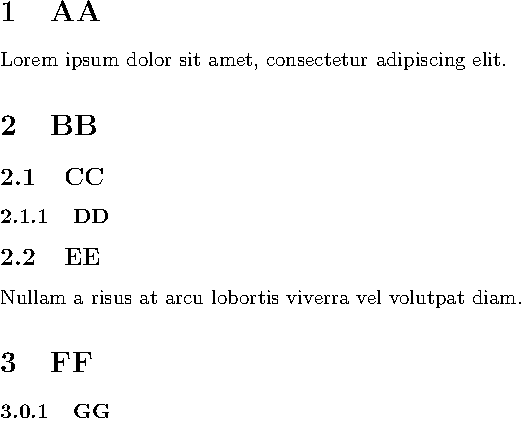
\includegraphics[width=\linewidth,height=0.8\textheight,keepaspectratio]{assets/sectioncommands.pdf}
			\end{column}
		\end{columns}
	\end{frame}

	\updatehighlight{
		name=accentB,
		remove={\section},
		add={\tableofcontents},
		%
		name=default,
		add={\section}
	}

	\begin{saveblock}{tableOfContents}
		\begin{highlightblock}[linewidth=0.5\textwidth,gobble=12]
			\begin{document}
				\maketitle
				\tableofcontents

				\section{AA}
				...
			\end{document}
		\end{highlightblock}
	\end{saveblock}

	\addtorecentlist{\textbackslash tableofcontents}

	\begin{frame}
		\frametitle{Inhoudsopgave}
		
		\begin{columns}
			\begin{column}{0.5\textwidth}
				\useblock{tableOfContents}
			\end{column}
			\begin{column}{0.5\textwidth}
				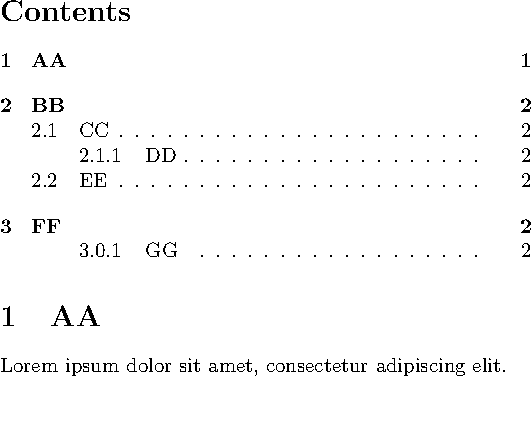
\includegraphics[width=\linewidth,height=0.8\textheight,keepaspectratio,page=1]{assets/tableofcontents.pdf}
			\end{column}
		\end{columns}
	\end{frame}

	\begin{saveblock}{tableOfContents}
		\begin{highlightblock}[linewidth=0.5\textwidth,gobble=12]
			\begin{document}
				\maketitle
				\tableofcontents
				\newpage
				
				\section{AA}
				...
			\end{document}
		\end{highlightblock}
	\end{saveblock}

	\addtorecentlist{\textbackslash newpage}
	\begin{frame}
		\frametitle{Inhoudsopgave}
		
		\begin{columns}
			\begin{column}{0.5\textwidth}
				\useblock{tableOfContents}
			\end{column}
			\begin{column}{0.5\textwidth}
				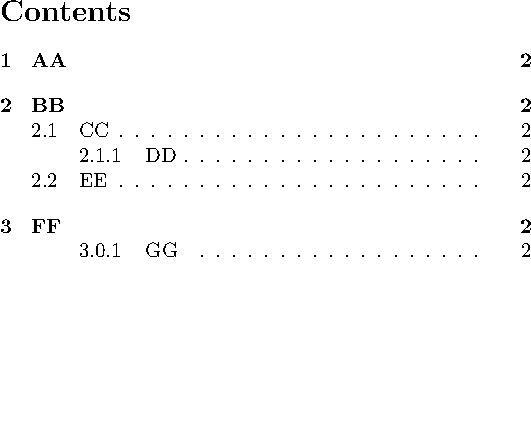
\includegraphics[width=\linewidth,height=0.8\textheight,keepaspectratio,page=1]{assets/tableofcontentswholepage.pdf}
			\end{column}
		\end{columns}
	\end{frame}

	\begin{saveblock}{tableOfContents}
		\begin{highlightblock}[linewidth=0.5\textwidth,gobble=12]
			...
			\usepackage[dutch]{babel}
			
			\begin{document}
				\maketitle
				\tableofcontents
				\newpage
				
				\section{AA}
				...
			\end{document}
		\end{highlightblock}
	\end{saveblock}
	
	\addtorecentlist{babel}
	
	\begin{frame}
		\frametitle{Inhoudsopgave}
		
		\begin{columns}
			\begin{column}{0.5\textwidth}
				\useblock{tableOfContents}
			\end{column}
			\begin{column}{0.5\textwidth}
				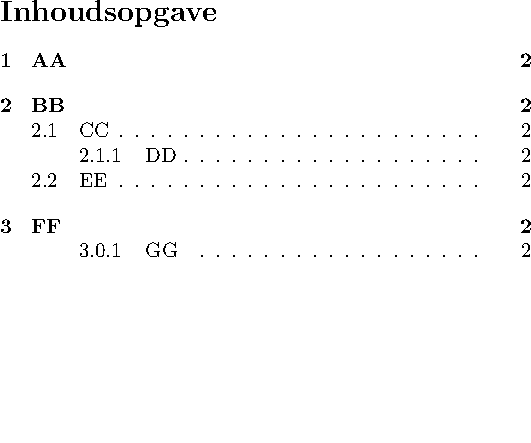
\includegraphics[width=\linewidth,height=0.8\textheight,keepaspectratio,page=1]{assets/tableofcontentsdutch.pdf}
			\end{column}
		\end{columns}
	\end{frame}

	\updatehighlight{
		name=accentB,
		add={\section},
	}

	\addtorecentlist{\textbackslash section*}

	\begin{frame}
		\frametitle{Genummerd}
		
		\begin{columns}
			\begin{column}{0.5\textwidth}
				\useblock{sectionCommands}
			\end{column}
			\begin{column}{0.5\textwidth}
				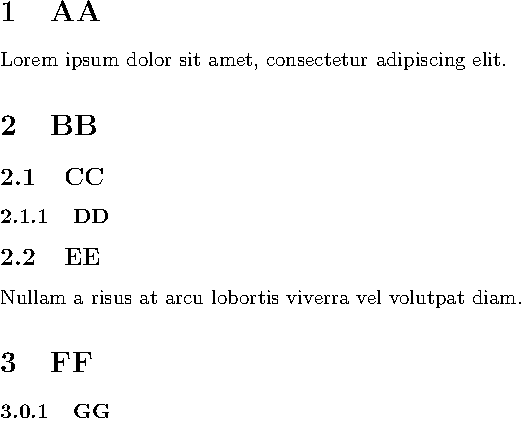
\includegraphics[width=\linewidth,height=0.8\textheight,keepaspectratio]{assets/sectioncommands.pdf}
			\end{column}
		\end{columns}
	\end{frame}

	\begin{saveblock}{partialNumbered}
		\begin{highlightblock}[linewidth=0.5\textwidth,gobble=12]
			\section{AA}
			Lorem ipsum dolor sit amet,
			consectetur adipiscing elit.
			
			\section*{BB}
			\subsection*{CC}
			\subsubsection{DD}
			\subsection*{EE}
			Nullam a risus at arcu
			lobortis viverra vel
			volutpat diam.
			
			\section{FF}
			\subsubsection{GG}
		\end{highlightblock}
	\end{saveblock}

	\begin{frame}
		\frametitle{Deels genummerd}
		
		\begin{columns}
			\begin{column}{0.5\textwidth}
				\useblock{partialNumbered}
			\end{column}
			\begin{column}{0.5\textwidth}
				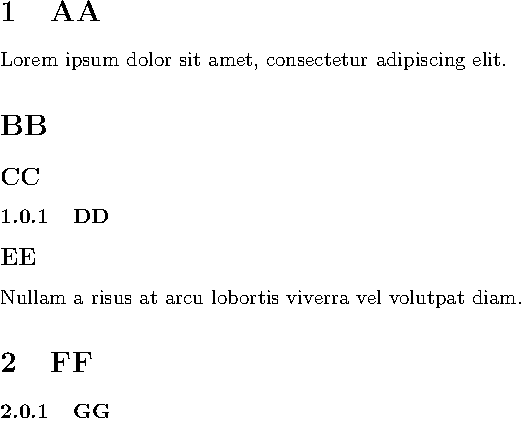
\includegraphics[width=\linewidth,height=0.8\textheight,keepaspectratio]{assets/partialNumberedStars.pdf}
			\end{column}
		\end{columns}
	\end{frame}

	\addtorecentlist{secnumdepth}

	\begin{frame}
		\frametitle{Genummerd}
		
		\begin{columns}
			\begin{column}{0.5\textwidth}
				\useblock{sectionCommands}
			\end{column}
			\begin{column}{0.5\textwidth}
				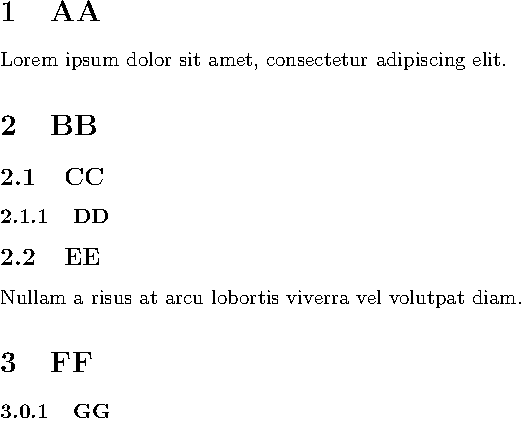
\includegraphics[width=\linewidth,height=0.8\textheight,keepaspectratio]{assets/sectioncommands.pdf}
			\end{column}
		\end{columns}
	\end{frame}

	\begin{saveblock}{partialNumbered}
		\begin{highlightblock}[linewidth=0.5\textwidth,gobble=12]
			\setcounter{secnumdepth}{2}
			\section{AA}
			Lorem ipsum dolor sit amet,
			consectetur adipiscing elit.
			
			\section{BB}
			\subsection{CC}
			\subsubsection{DD}
			\subsection{EE}
			Nullam a risus at arcu
			lobortis viverra vel
			volutpat diam.
			
			\section{FF}
			\subsubsection{GG}
		\end{highlightblock}
	\end{saveblock}
	
	\begin{frame}
		\frametitle{Deels genummerd}
		
		\begin{columns}
			\begin{column}{0.5\textwidth}
				\useblock{partialNumbered}
			\end{column}
			\begin{column}{0.5\textwidth}
				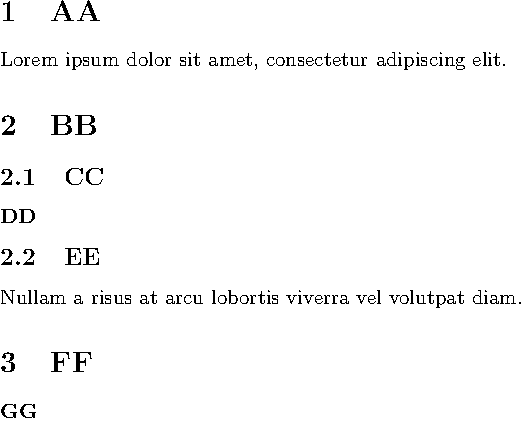
\includegraphics[width=\linewidth,height=0.8\textheight,keepaspectratio]{assets/partialNumberedSecnumdepth2.pdf}
			\end{column}
		\end{columns}
	\end{frame}

	\begin{saveblock}{partialNumbered}
		\begin{highlightblock}[linewidth=0.5\textwidth,gobble=12]
			\setcounter{secnumdepth}{1}
			\section{AA}
			Lorem ipsum dolor sit amet,
			consectetur adipiscing elit.
			
			\section{BB}
			\subsection{CC}
			\subsubsection{DD}
			\subsection{EE}
			Nullam a risus at arcu
			lobortis viverra vel
			volutpat diam.
			
			\section{FF}
			\subsubsection{GG}
		\end{highlightblock}
	\end{saveblock}
	
	\begin{frame}
		\frametitle{Deels genummerd}
		
		\begin{columns}
			\begin{column}{0.5\textwidth}
				\useblock{partialNumbered}
			\end{column}
			\begin{column}{0.5\textwidth}
				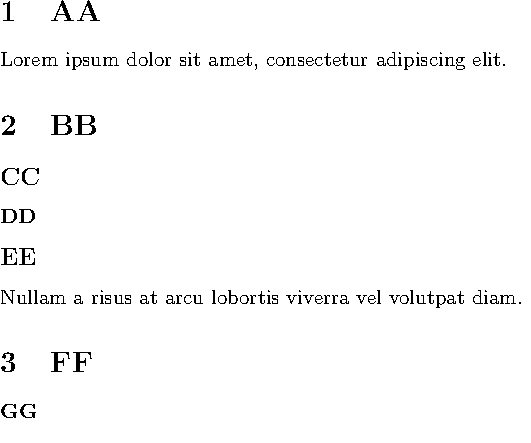
\includegraphics[width=\linewidth,height=0.8\textheight,keepaspectratio]{assets/partialNumberedSecnumdepth1.pdf}
			\end{column}
		\end{columns}
	\end{frame}

	\begin{saveblock}{partialNumbered}
		\begin{highlightblock}[linewidth=0.5\textwidth,gobble=12]
			\setcounter{secnumdepth}{0}
			\section{AA}
			Lorem ipsum dolor sit amet,
			consectetur adipiscing elit.
			
			\section{BB}
			\subsection{CC}
			\subsubsection{DD}
			\subsection{EE}
			Nullam a risus at arcu
			lobortis viverra vel
			volutpat diam.
			
			\section{FF}
			\subsubsection{GG}
		\end{highlightblock}
	\end{saveblock}
	
	\begin{frame}
		\frametitle{Ongenummerd}
		
		\begin{columns}
			\begin{column}{0.5\textwidth}
				\useblock{partialNumbered}
			\end{column}
			\begin{column}{0.5\textwidth}
				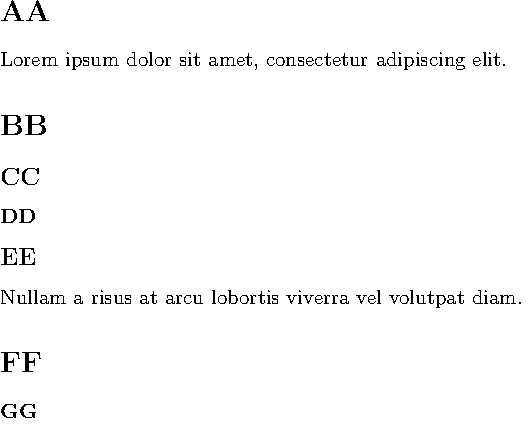
\includegraphics[width=\linewidth,height=0.8\textheight,keepaspectratio]{assets/partialNumberedSecnumdepth0.pdf}
			\end{column}
		\end{columns}
	\end{frame}
\end{document}
